% Euler line OGH and the nine-point circle (centre N, radius R/2); all nine points checked to 1e-12.
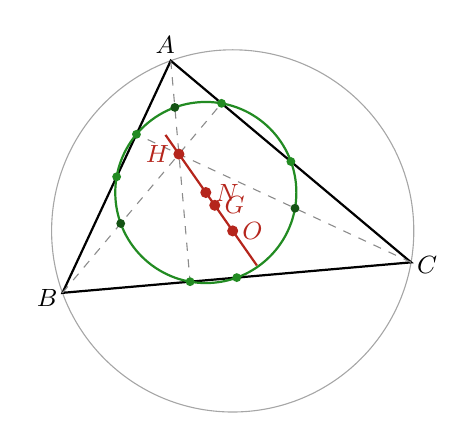
\begin{tikzpicture}[font=\small]
\draw[black!35] (0,0) circle (2.300);
\draw[thick] (-0.7866,2.1613) -- (-2.1613,-0.7866) -- (2.2651,-0.3994) -- cycle;
\draw[black!45,dashed] (-0.7866,2.1613) -- (-0.5411,-0.6449);
\draw[black!45,dashed] (-2.1613,-0.7866) -- (-0.1417,1.6202);
\draw[black!45,dashed] (2.2651,-0.3994) -- (-1.2224,1.2268);
\draw[ForestGreen,thick] (-0.3414,0.4876) circle (1.150);
\draw[BrickRed,thick] (0.3073,-0.4389) -- (-0.8536,1.2191);
\fill[ForestGreen] (-0.5411,-0.6449) circle (1.6pt);
\fill[ForestGreen] (-0.1417,1.6202) circle (1.6pt);
\fill[ForestGreen] (-1.2224,1.2268) circle (1.6pt);
\fill[ForestGreen] (0.0519,-0.5930) circle (1.6pt);
\fill[ForestGreen] (0.7392,0.8810) circle (1.6pt);
\fill[ForestGreen] (-1.4740,0.6873) circle (1.6pt);
\fill[ForestGreen!60!black] (-0.7348,1.5683) circle (1.6pt);
\fill[ForestGreen!60!black] (-1.4221,0.0943) circle (1.6pt);
\fill[ForestGreen!60!black] (0.7911,0.2879) circle (1.6pt);
\fill[BrickRed] (0.0000,0.0000) circle (2pt) node[right,BrickRed] {$O$};
\fill[BrickRed] (-0.2276,0.3251) circle (2pt) node[right,BrickRed] {$G$};
\fill[BrickRed] (-0.3414,0.4876) circle (2pt) node[right,BrickRed] {$N$};
\fill[BrickRed] (-0.6829,0.9753) circle (2pt) node[left,BrickRed] {$H$};
\node at (-0.8574,2.3558) {$A$};
\node at (-2.3558,-0.8574) {$B$};
\node at (2.4689,-0.4353) {$C$};
\end{tikzpicture}
